\documentclass{article}
\usepackage[utf8]{inputenc}

\usepackage{graphicx,caption}
\graphicspath{ {./images/} }
\usepackage{float}
\usepackage{caption}
\usepackage{subcaption}
\usepackage[unicode]{hyperref}
\usepackage{amsmath}
\usepackage[shortlabels]{enumitem}

\usepackage{listings}
\usepackage{xcolor}
\definecolor{codegreen}{rgb}{0,0.6,0}
\definecolor{codegray}{rgb}{0.5,0.5,0.5}
\definecolor{codepurple}{rgb}{0.58,0,0.82}
\definecolor{backcolour}{rgb}{0.95,0.95,0.92}
 \lstdefinestyle{mystyle}{
    backgroundcolor=\color{backcolour},   
    commentstyle=\color{codegreen},
    keywordstyle=\color{black},
    numberstyle=\tiny\color{codegray},
    stringstyle=\color{codepurple},
    basicstyle=\ttfamily\footnotesize,
    breakatwhitespace=false,         
    breaklines=true,                 
    captionpos=b,                    
    keepspaces=true,                 
    numbers=left,                    
    numbersep=5pt,                  
    showspaces=false,                
    showstringspaces=false,
    showtabs=false,                  
    tabsize=2
}
\lstset{style=mystyle}

\title{Homework 5 - Theory/Laboratory}
\author{Dainese Fabio, 857661}
\date{April 12, 2020}

\begin{document}

\maketitle

\section{The Watts and Strogatz’s Model}
    \begin{itemize}
        \item The local \textit{clustering coefficient} (CC),  provided in the \textit{Watts and Strogatz} paper, measures the cliquishness of a neighbourhood (you can see this feature also as how likely 2 nodes that are connected are part of some larger highly connected group of node - i.e. clique).\newline
        
        \par\noindent This statistic can assume values between 0 and 1, indicating the fraction of possible interconnections between the neighbours of a node (visually you can consider that 0 indicate a start topology graph, meanwhile 1 means a clique).\newline
        
        \par\noindent To compute the CC of a graph you just need to consider the average value between all the CC of each node belonging to the graph.
        
    
        \item Considering the scenario of having \(n = 400\) nodes, \(K = 10\) and the re-wiring probability \(q = 0.01 + 0.01j\), for \(j = 1,...,99\). \newline
        
        \par\noindent The average clustering coefficient (CC(q)) and the average path length (APL(q)) for each \(q\) has been calculated using the following \textit{MatLab} code:\newline
        
        \begin{lstlisting}[language=Matlab]
clear all;
clc;

n = 400;
K = 10;

q_cumulative = (0.02:0.01:1)';
q_length = size(q_cumulative,1);
storage = zeros(q_length,2);

for j=1:q_length
    q = q_cumulative(j,1);
    WS = WattsStrogatz(n,K,q);
    cc = clustering_coef_bu(WS.adjacency);
    
    storage(j,1) = mean(cc);
    storage(j,2) = mean(distances(WS),'all');
end

figure(1)
plot(q_cumulative,storage(:,1),'k-');
title('CC(q)');
xlabel('Re-wiring probability');
ylabel('Clustering coefficient');

figure(2)
plot(q_cumulative,storage(:,2),'k-');
title('APL(q)');
xlabel('Re-wiring probability');
ylabel('Average path length');
\end{lstlisting}
        
        \noindent Which generates the following two graphs:
        
        \begin{figure}[H]
            \centering
            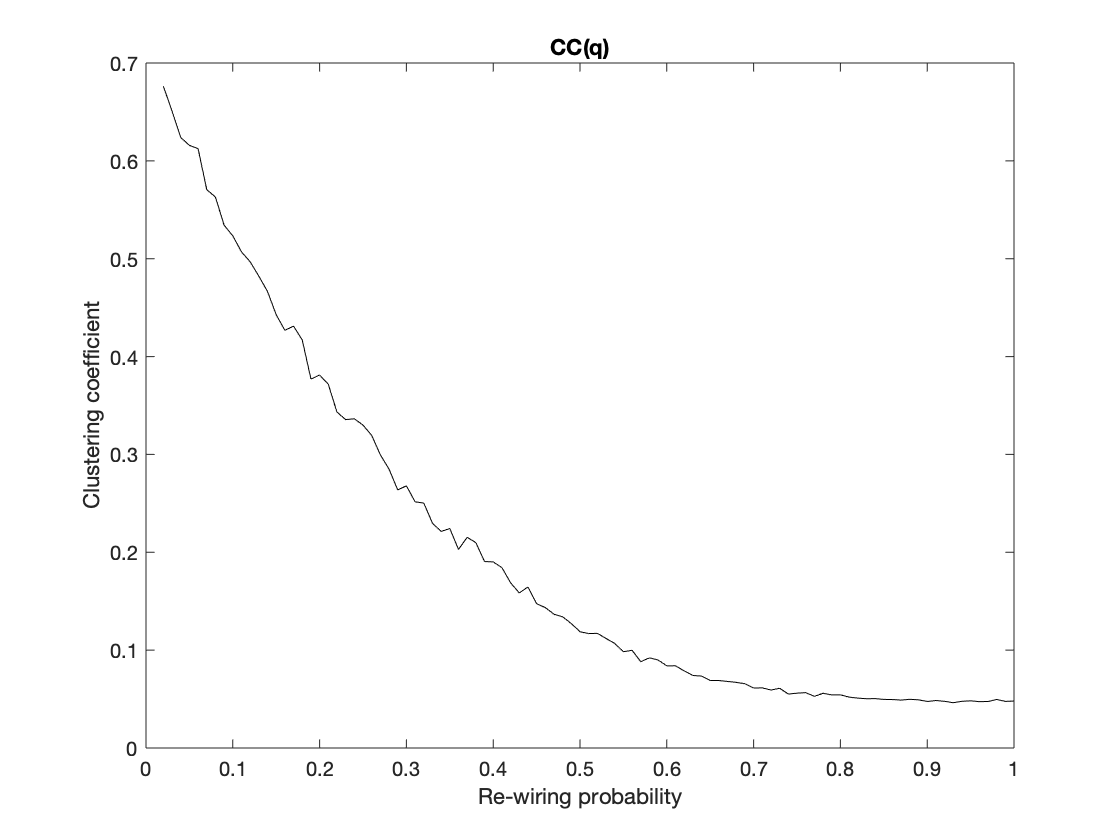
\includegraphics[width=0.9\textwidth]{1.png}
            \caption{Average clustering coefficient}
            \label{fig:figure-1}
        \end{figure}
        \begin{figure}[H]
            \centering
            
            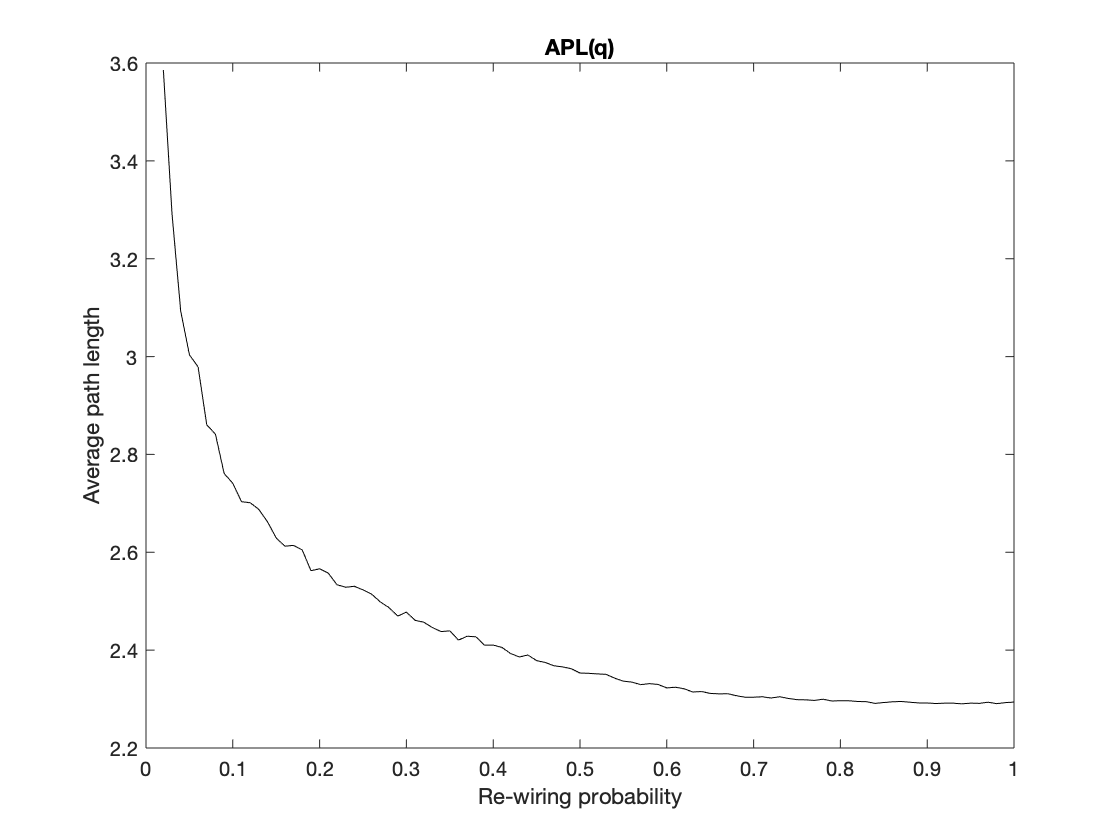
\includegraphics[width=0.9\textwidth]{2.png}
            \caption{Average path length}
            \label{fig:figure-2}
        \end{figure}
        
        \item By setting the logarithmic horizontal scale to the previous graphs it has been more clear that the \(APL(q)\) drops very quickly (meaning that thanks to the re-wiring process the distance between the nodes in the network decreased), meanwhile the \(CC(q)\) at the beginning (regular lattice 'state') decrease very slowly, indicating that the transition to a small world is almost undetectable at the local level.

    \end{itemize}

\end{document}
